% !TeX program = xelatex
% 本文档基于 ctexart(scheme=chinese) + xeCJK，必须使用 XeLaTeX 编译；
% 若用 pdflatex 编译，会在附录 C 的代码环境处因中文字符而报错退出。
%
% ------------------------------------------------------------
% 文件结构说明（便于 navigation）：
% 本文件只保留 LaTeX 导言区（宏包/排版设置）与章节装配顺序，
% 每个 \section 级别的实际内容拆分到 sections/ 目录下的独立 .tex 文件中，
% 文件名前缀数字即正文出现顺序。写作/编辑某一章时直接打开对应的
% sections/XX_xxx.tex，不需要在几百行的单一文件里滚动查找。
% 新增/调整章节顺序时，只需要在下方的装配区调整 \input 顺序，
% 不需要搬动章节内容本身。
% ------------------------------------------------------------
\documentclass[12pt, a4paper, scheme=chinese, fontset=windows]{ctexart}

% ---------------- 字体 ----------------
% 全文正文字体固定为宋体；宋体本身没有真正的粗体字重，\bfseries 默认只是
% "伪粗体"（描边加粗），标题/强调文字观感很弱。这里显式把粗体字重指向黑体，
% 使 \bfseries、\textbf{} 在保持宋体正文的同时获得清晰可辨的粗体效果。
\setCJKmainfont[BoldFont=SimHei]{SimSun}

% ---------------- 页面与基础排版 ----------------
\usepackage[a4paper, top=2.5cm, bottom=2.5cm, left=2.4cm, right=2.4cm]{geometry}
\usepackage{setspace}
\setstretch{1.35}                 % 行距，可按赛区要求调整（常见 1.25~1.5）
\usepackage{indentfirst}
\setlength{\parindent}{2em}

% ---------------- 数学与符号 ----------------
\usepackage{amsmath, amssymb, amsfonts, bm}

% ---------------- 表格 ----------------
\usepackage{booktabs}
\usepackage{array}
\usepackage{multirow}
\usepackage{longtable}
\usepackage{caption}
\captionsetup{font=small, labelfont=bf}
\usepackage{subcaption}

% ---------------- 图片与占位框 ----------------
\usepackage{graphicx}
\usepackage{float}
\usepackage{tikz}
% 占位图：正式提交前请替换为 \includegraphics[width=..]{图片路径}
% 用法：\FigPlaceholder{宽cm}{高cm}{占位说明文字}——说明文字仅作占位提示，
% 图号/图题请统一交给下方的 \caption 生成，避免出现重复编号。
\newcommand{\FigPlaceholder}[3]{%
  \begin{tikzpicture}
    \useasboundingbox (0,0) rectangle (#1,#2);
    \draw[dashed, gray] (0,0) rectangle (#1,#2);
    \node[align=center, text width=#1 cm, gray] at (#1/2,#2/2) {#3};
  \end{tikzpicture}%
}

% ---------------- 列表 ----------------
\usepackage{enumitem}
\setlist[itemize]{leftmargin=2em, itemsep=0.2em}
\setlist[enumerate]{leftmargin=2.4em, itemsep=0.2em}

% ---------------- 代码环境（用于附录代码展示）----------------
\usepackage{xcolor}
\usepackage{listings}
\lstdefinestyle{pystyle}{
  language=Python,
  basicstyle=\ttfamily\small,
  keywordstyle=\color{blue!70!black}\bfseries,
  commentstyle=\color{gray}\itshape,
  stringstyle=\color{orange!70!black},
  numbers=left,
  numberstyle=\tiny\color{gray},
  numbersep=6pt,
  frame=single,
  breaklines=true,
  breakatwhitespace=false,
  showstringspaces=false,
  tabsize=4,
  columns=flexible,
  extendedchars=true,
}
\lstset{style=pystyle}

% ---------------- 超链接（隐藏彩色边框，便于打印）----------------
\usepackage[hidelinks]{hyperref}

% ---------------- 页眉页脚 ----------------
\pagestyle{plain}

% ---------------- 标题编号：一、二、三…（章）+ 4.1（节）----------------
% ctexart 的 scheme=chinese 不会自动把 \section 编号改成中文数字，
% 这里显式覆盖 \thesection，使其呈现为样例论文中的“一、”“二、”…风格；
% \subsection / \subsubsection 保持阿拉伯数字（如 4.1、4.3.1），与样例一致。
\renewcommand{\thesection}{\chinese{section}、}
% 注意：\subsection/\subsubsection 默认引用 \thesection 作为前缀，
% 这里显式改回阿拉伯数字前缀（如 4.1、4.3.1），避免变成“一、.1”。
\renewcommand{\thesubsection}{\arabic{section}.\arabic{subsection}}
\renewcommand{\thesubsubsection}{\arabic{section}.\arabic{subsection}.\arabic{subsubsection}}
\ctexset{
  section = {
    format     += \Large\bfseries,
    aftername   = {},
    numbering   = true,
  }
}

% ============================================================
\begin{document}

% ------------------------------------------------------------
% 章节装配区：按正文出现顺序 \input 对应文件，不在此处直接写正文内容。
% 每个文件对应一个 \section 级别的章节，文件名前缀数字
% 即装配顺序，调整顺序时改这里的排列即可，不需要搬动章节内容。
% ------------------------------------------------------------
% ============================================================
% 标题 + 摘要 + 关键词
% ------------------------------------------------------------
% 说明：全国大学生数学建模竞赛的封面由组委会统一提供（含题目、
% 参赛队号、密封线等），正文一般从「摘要」开始单独编排。
% 如需要自制封面，可在此处插入 titlepage，比赛提交时请按实际要求删除/替换。
% ------------------------------------------------------------

\begin{center}
  {\zihao{3}\bfseries [论文题目]}
\end{center}

\vspace{1em}
\begin{center}
  {\zihao{-2}\bfseries 摘\quad 要}
\end{center}

\noindent
% ------------------------------------------------------------
% 摘要写作要点（参考样例论文 C023）：
% 1. 一句话点出问题背景与研究对象；
% 2. 概述总体建模思路（用了什么方法框架）；
% 3. 分问题逐段说明「做了什么 —— 用什么方法 —— 得到什么结果（含关键数字）」；
% 4. 末段点出创新点 / 应用价值。
% ------------------------------------------------------------
【占位：一段总起，交代问题背景、研究对象与总体建模框架。】

\textbf{针对问题一，}【占位：方法 + 关键结果】。

\textbf{针对问题二，}【占位：方法 + 关键结果】。

\textbf{针对问题三，}【占位：方法 + 关键结果】。

\textbf{针对问题四，}【占位：方法 + 关键结果】。

【占位：总结全文创新点，如模型融合思路、算法设计、可视化/工程实现等。】

\vspace{0.6em}
\noindent\textbf{关键词：} [关键词1]\quad [关键词2]\quad [关键词3]\quad [关键词4]\quad [关键词5]

\newpage
      % 标题 + 摘要 + 关键词
% ============================================================
\section{问题重述}

\subsection{问题背景}
% 写作结构建议：背景现状 -> 已有解决方案/技术 -> 现存问题与不足 -> 本文研究的意义
【占位：介绍问题所处的现实背景，说明当前已有的方法/方案是什么。】

【占位：指出现有方案存在的局限性、痛点或尚未解决的问题。】

【占位：说明科学、准确地解决该问题对实际应用/决策的重要意义，引出本文工作。】

\subsection{问题要求}
本研究需结合所提供的数据，建立数学模型以系统研究以下问题：

\textbf{问题1} 【占位：复述题目问题一的核心要求】。

\textbf{问题2} 【占位：复述题目问题二的核心要求】。

\textbf{问题3} 【占位：复述题目问题三的核心要求】。

\textbf{问题4} 【占位：复述题目问题四的核心要求】。
       % 一、问题重述
% ============================================================


\section{问题分析}

在展开具体建模之前，先明确本文所研究微网整体结构及主要能量流关系，如图\ref{fig:relationship}。


\begin{figure}[H]
  \centering
  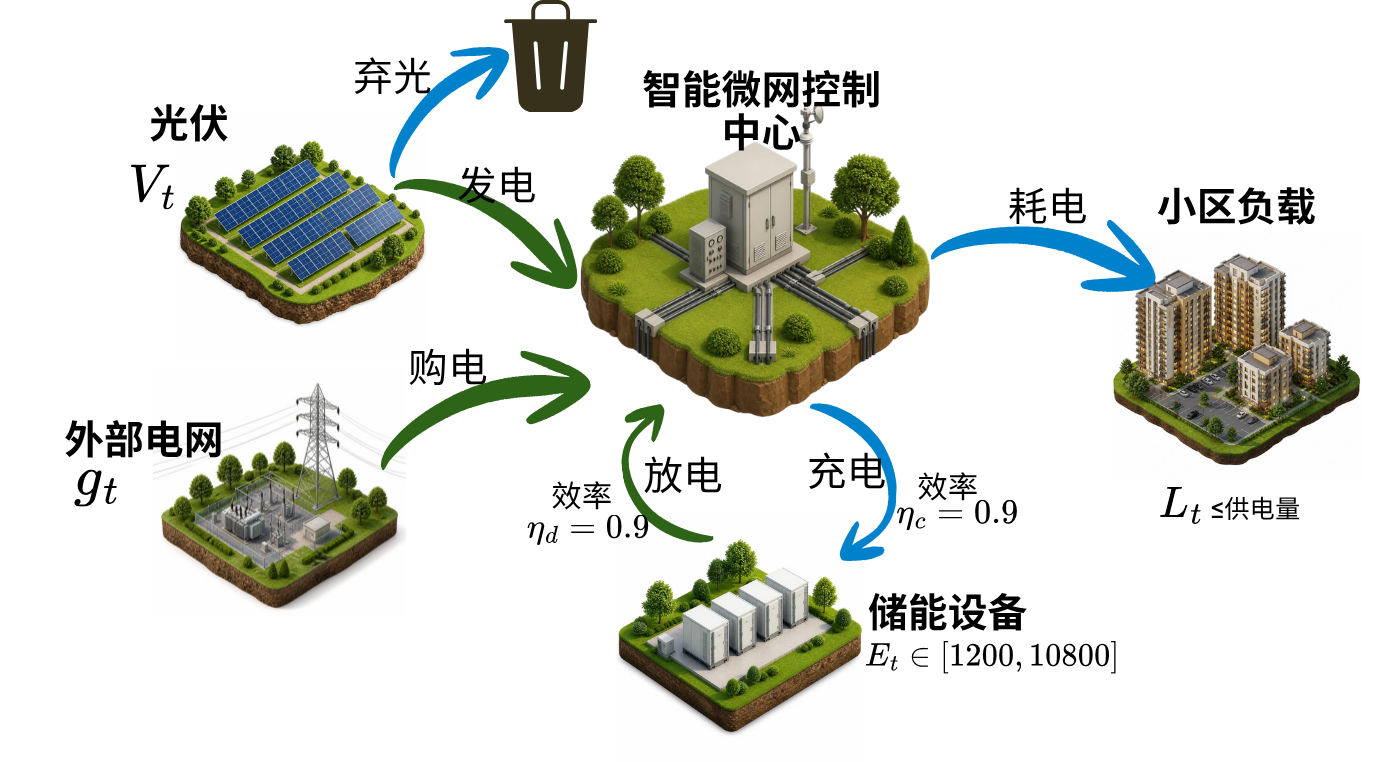
\includegraphics[width=0.70\linewidth]{figures/relationship.png}
  \caption{微网系统中光伏、外网、储能与小区负载间的能量流关系}
  \label{fig:relationship}
\end{figure}

控制中心统一调度光伏、外网购电两路输入及储能充放电，供给小区负荷；后续各问均围绕这一能量流展开，差异体现在决策时点、信息可得性与约束条件上。本文由确定性调度出发，逐步考虑预测不确定性、日内滚动调整及动态电价下的跨日决策，形成如下总体研究思路：

\begin{figure}[H]
  \centering
  \includegraphics[width=0.85\linewidth]{figures/our_work.png}
  \caption{总体研究思路流程图}
  \label{fig:overall-flow}
\end{figure}
      % 二、问题分析
% ============================================================
\section{模型假设}

为简化问题、聚焦核心矛盾，本文做出以下假设：

\textbf{假设1：} 将进入日内调度与执行的负荷、光伏功率及电价序列统一离散到10 min时间尺度。在每个调度时段内，各变量采用该时段的代表值，忽略时段内部的短时波动；功率对应的时段电量按
\[
E_t=P_t\Delta t,\qquad \Delta t=\frac{1}{6}\text{ h}
\]
计算，购电费用按各类购电量与其对应结算单价计算。

\textbf{假设2：} 将小区微网等效为聚合能源系统，仅在系统总量层面考虑负荷、光伏发电、外网购电、储能充放电及弃光等能量流动；对于不同问题中涉及的调整购电、紧急购电等方式，均纳入相应时段的总能量平衡。忽略配电网内部线路损耗、节点电压及潮流分布等空间因素。

\textbf{假设3：} 对储能性能的时间变化作短期稳定化处理。在研究周期内，储能系统的容量边界、充放电功率上限及充放电效率按题目给定值和模型设定的固定值处理，不考虑温度变化、设备老化、自放电及故障等因素引起的变化。

\textbf{假设4：} 在每个调度或滚动决策时刻，模型规定可使用的历史观测、当前储电量及已发布预报能够及时、准确获得，且调度指令能够在相应时段内执行，忽略测量误差、通信延迟和控制执行滞后；对于决策时尚未知的未来信息，仍按照各问题所建立的预测或估计方法处理。
   % 三、模型假设
% ============================================================
\section{符号说明}
\begin{table}[H]
  \centering
  \label{tab:notation}
  \footnotesize
  \renewcommand{\arraystretch}{1.05}
  \begin{tabular}{cll}
    \toprule
    符号 & 说明 & 单位 \\
    \midrule
    $t$ & 10分钟时段编号，$t=1,\ldots,144$ & -- \\
    $d$ & 日期编号（滚动预测/调度的当前天） & -- \\
    $p_t$ & 时段 $t$ 的购电电价 & 元/kWh \\
    $L_t$ & 时段 $t$ 的负载电量 & kWh \\
    $V_t$ & 时段 $t$ 的光伏预测电量 & kWh \\
    $g_t,\,g_t^0$ & 时段 $t$ 的（原）计划购电量 & kWh \\
    $c_t,\,d_t$ & 储能设备外部端口的充电量、放电量 & kWh \\
    $w_t$ & 未利用（弃用）的光伏电量 & kWh \\
    $E_t,\,E_0,\,E_{\mathrm{end}}$ & 时段 $t$末、初始（0:00）、当天24:00的储能电量 & kWh \\
    $\eta_c,\,\eta_d$ & 储能充电效率、放电效率 & 无量纲 \\
    $z_t$ & 储能充电模式二元变量（1为充电、0为放电） & 0/1 \\
    $M_c,\,M_d$ & 单时段最大充电电量、最大放电电量 & kWh \\
    $F,\,F_{\mathrm{LP}}^\ast,\,F_{\mathrm{MILP}}^\ast$ & 全天购电费用（目标函数）、LP松弛与原MILP最优值 & 元 \\
    $u_t,\,v_t$ & 日内调整中购电量的追加量、减购量 & kWh \\
    $h_t,\,h_t^{(j)}$ & 实际（或按情景 $j$ 计）发生的紧急购电量 & kWh \\
    $a_t,\,a_t^{(j)}$ & 净负荷电量、按历史误差情景 $j$ 构造的净负荷情景 & kWh \\
    $C,\,C_{\mathrm{purchase}},\,C_{\mathrm{opt}}$ & 全年总费用、购电类费用合计、带惩罚项的优化目标 & 元 \\
    $W$ & 净负荷预测模型的滚动训练窗口长度 & 天 \\
    $K_L,\,K_P$ & 负荷、光伏PCA保留的主成分个数 & -- \\
    $\widehat{\bm L}_d,\,\widehat{\bm P}_d$ & 第 $d$ 天负荷、光伏曲线的中心预测 & kWh \\
    $q,\,q^\ast$ & 计划购电所依据的净负荷风险分位数、开发期扫描确定的最优值 & -- \\
    $\tau$ & 光伏预报发布时刻（00:00/06:00/12:00/18:00） & 时:分 \\
    $x$ & 期末可用储能量（以容量下限1200\,kWh为基准） & kWh \\
    \bottomrule
  \end{tabular}
\end{table}
      % 四、符号说明
% ============================================================
\section{数据处理}
% 本章只做全局性的数据画像：来源、规模、变量字典、整体数据质量，以及对所有问题
% 都成立的通用处理约定（如时段编号方式）——不做面向具体某一问建模需求的清洗/
% 特征决策，那些放在各问求解章各自的“N.1 数据预处理”小节中。5.1 只说明数据
% 本身长什么样，5.2 说明为了让全部问题能在统一口径下使用这批数据而做的通用处理。

\subsection{数据说明}
本题数据由题目附件1至附件4提供，均为微网运行相关的时间序列数据，采样粒度统一为10分钟（每天144个时段）。附件1给出某一典型日全天的电价、小区负载与光伏预测功率，共\textbf{144条记录}；附件2给出2025年全年每天的小区负载与光伏发电实际功率，共\textbf{52{,}560条记录}；附件3给出2025年全年每天0:00、6:00、12:00、18:00共四个时刻发布的未来24小时整点光伏发电功率预报，累计\textbf{35{,}040条}原始整点预报记录；附件4给出2025年全年每天不同时间的实际电价，同样为\textbf{52{,}560条记录}。

\subsection{数据处理}
为便于各问在统一口径下调用同一批数据，本文对原始数据做了时段编号处理。将每天划分为$t=1,2,\ldots,144$共144个时段，第$t$个时段对应的时间区间为
\begin{equation}
I_t=\big[(t-1)\Delta t,\ t\Delta t\big),\qquad \Delta t=\tfrac16\ \text{小时（10分钟）}.
\end{equation}
即时段$t$覆盖当天第$(t-1)\times10$分钟至第$t\times10$分钟。全年数据按来源日期与$t=1,\ldots,144$关联，某日24:00的采样仍归属当天（不归入次日），从而保证同一天的144个时段构成一个完整、无重叠的日历日。  % 五、数据侧写
% ============================================================
\section{问题一的求解}

\subsection{问题一的数据预处理}
【占位：仅说明为回答问题一而对数据侧写章节所述数据做的针对性处理——如筛选本问
所需的变量子集、本问特有的缺失值/异常值处理策略、特征构造/离散化、标准化方式等，
并说明选择依据。全局性、对所有问都成立的处理已在“数据侧写”章交代，此处不重复。】
            % 六、问题一的求解
% ============================================================
\section{问题二的求解}

\subsection{问题二的数据预处理}
【占位：同上，仅说明针对问题二的数据处理决策。】
            % 七、问题二的求解
% ============================================================
\section{问题三的求解}

\subsection{问题三的数据预处理}
【占位：同上，仅说明针对问题三的数据处理决策。】
            % 八、问题三的求解
% ============================================================
\section{问题四的求解}

\subsection{问题四的数据预处理}
【占位：同上，仅说明针对问题四的数据处理决策。】
            % 九、问题四的求解
% ============================================================
\section{模型的评价、改进与推广}

\subsection{模型的优点}

\begin{enumerate}
  \item \textbf{物理对象和决策时序保持统一。}
  模型围绕负荷、光伏、外网购电和储能建立总量能量平衡，并在各问中连续传递储能状态。统一的状态和能量口径使不同信息条件下的调度方案具有可比性，也便于检查方案是否满足基本物理约束。

  \item \textbf{建模边界与信息条件相匹配。}
  模型根据决策时点能够获得的信息安排预测、计划和调整环节，在保留共同物理结构的同时，分别处理输入不确定性、日内更新和跨日状态传递，避免用同一组信息假定覆盖所有决策阶段。

  \item \textbf{同时检查经济指标与可行性。}
  各方案以购电及相关附加费用作为主要经济指标，同时复核能量平衡、储能状态、容量和功率边界。经济指标与约束校验同时保留，使评价既能反映运行成本，也能排除不可执行的调度结果。

  \item \textbf{显式表示储能的跨日作用。}
  问题四将日末储能保留量对后续运行的影响表示为终端价值，并在日前计划和日内滚动调整中使用，使储能决策不再局限于单日费用最小化。
\end{enumerate}

\subsection{模型的不足}

\begin{enumerate}
  \item \textbf{聚合模型未描述配电网空间约束。}
  当前模型将小区视为单一聚合节点，未考虑节点电压、线路容量、潮流分布和线路损耗；当局部网络约束成为主要瓶颈时，模型可能低估实际运行限制。

  \item \textbf{储能模型未计入全生命周期因素。}
  模型按固定性能参数描述储能，未考虑温度、老化、自放电、健康状态和循环退化成本。因此，费用结果主要反映运行阶段的购电成本，不等同于储能设备的全生命周期经济收益。

  \item \textbf{预测模型依赖历史规律，面对突发变化的能力有限。}
  问题二、三使用历史信息构造负荷和光伏预测场景，问题四的电价采用前一周同日同刻预测。面对节假日、天气突变或价格机制变化时，历史规律可能不足以代表当前情形，且本文未建立完整的电价概率预测。

  \item \textbf{终端价值和实际执行仍是近似处理。}
  问题四的终端价值由有限预测视野、有限储能取点和小时聚合估计。问题三以及问题四的滚动方案会在规定决策时刻重新优化计划，但这些过程仍是在历史数据上的离线回测，执行阶段按照代码设定的实际供需替换和富余先充、缺口先放规则运行，尚未接入真实能源管理系统进行在线数据采集、控制下发和闭环运行。
\end{enumerate}

\subsection{模型的改进与推广}

\begin{enumerate}
  \item \textbf{引入配电网网络约束。}
  对于园区或多节点微电网，可在现有能量平衡模型上增加节点、线路、潮流和电压约束，将聚合模型扩展为配电网最优潮流或线性化潮流模型。原有储能和费用目标可以保留，但网络参数需要根据实际拓扑重新估计。

  \item \textbf{加入储能退化和健康状态模型。}
  可在目标函数中加入循环退化成本，并根据充放电深度、温度和荷电状态建立分段线性退化模型；若有长期运行数据，还可进一步引入 SOH 状态变量。这样得到的目标将从单纯运行购电成本扩展为运行成本与寿命成本的综合权衡。

  \item \textbf{完善不确定性处理和终端价值估计。}
  可将负荷、光伏和电价的预测误差统一构造为带相关性的联合场景，并针对节假日、天气突变和价格异常增加校准机制；同时采用更细的时间粒度和更充分的储能状态取点估计终端价值，使其与滚动控制更紧密衔接。

  \item \textbf{拓展应用场景。}
  在补充网络拓扑、设备性能和运行数据后，本文的总量平衡与滚动调度思路可推广到园区微电网、工商业储能和光储充系统，也可扩展到多储能协调及需求响应问题。迁移时需要重新确定负荷、价格、储能和网络参数，并依据实际通信与控制条件重新检验可执行性。
\end{enumerate}
    % 十、模型的评价、改进与推广
% ============================================================
\section*{AI工具使用声明}
\addcontentsline{toc}{section}{AI工具使用声明}

本参赛队在竞赛过程中使用了AI工具，主要用于语言润色、代码调试等，
详细使用情况见支撑材料。
 % AI工具使用声明
% ============================================================
\begin{thebibliography}{99}
\bibitem{ref_curtailment} R. Hollinger, L. M. Diazgranados, T. Erge. Techno-economic analysis of battery storage and curtailment in a distribution grid with high PV penetration[J]. Journal of Energy Storage, 2018, 17: 73--83. DOI: 10.1016/j.est.2018.02.001.
\bibitem{ref_highs} Q. Huangfu, J. A. J. Hall. Parallelizing the dual revised simplex method[J]. Mathematical Programming Computation, 2018, 10(1): 119--142. DOI: 10.1007/s12532-017-0130-5.
\bibitem{ref_scipy} P. Virtanen, R. Gommers, T. E. Oliphant, et al. SciPy 1.0: fundamental algorithms for scientific computing in Python[J]. Nature Methods, 2020, 17(3): 261--272. DOI: 10.1038/s41592-019-0686-2.
\bibitem{ref_astra} OpenAI. GPT-6 Astra, ChatGPT (OpenAI)[EB/OL]. (2026-09-03). https://openai.com/index/advancing-the-price-performance-frontier-with-gpt-5-6/.
\bibitem{ref_deepseek} DeepSeek. DeepSeek-R1-0528, 深度求索（DeepSeek）[EB/OL]. (2025-05-28). https://api-docs.deepseek.com/updates/.
\end{thebibliography}    % 参考文献
\newpage
% ============================================================
\section*{附录A\quad 文件列表}
\begin{table}[H]
  \centering
  \caption{提交文件列表}
  \label{tab:appendix-files}
  \begin{tabular}{cl}
    \toprule
    文件名 & 功能描述 \\
    \midrule
    q1.py & 问题一程序代码 \\
    q2.py & 问题二程序代码 \\
    q3.py & 问题三程序代码 \\
    q4.py & 问题四程序代码 \\
    \bottomrule
  \end{tabular}
\end{table}

\section*{附录B\quad 部分数据展示}
【占位：展示原始数据或关键中间结果的部分样例，用于说明数据来源与建模输入的真实性。】

\begin{table}[H]
  \centering
  \caption{部分数据展示（示例）}
  \label{tab:appendix-data}
  \begin{tabular}{ccccc}
    \toprule
    编号 & 变量1 & 变量2 & 变量3 & 变量4 \\
    \midrule
    【占位】 & 【占位】 & 【占位】 & 【占位】 & 【占位】 \\
    【占位】 & 【占位】 & 【占位】 & 【占位】 & 【占位】 \\
    \bottomrule
  \end{tabular}
\end{table}

\section*{附录C\quad 代码}

% 方式一：直接内嵌代码（适合较短脚本，或需要展示核心片段时）
\subsection*{q1.py}
\begin{lstlisting}
# -*- coding: utf-8 -*-
"""
【占位：问题一核心代码，请替换为实际脚本内容】
"""
\end{lstlisting}

% 方式二：从外部文件直接引入完整代码（推荐，避免正文与代码文件不同步）
% 取消注释并将路径替换为你们的实际代码路径后使用：
% \lstinputlisting[language=Python, caption={q1.py}]{code/q1.py}
% \lstinputlisting[language=Python, caption={q2.py}]{code/q2.py}
% \lstinputlisting[language=Python, caption={q3.py}]{code/q3.py}
% \lstinputlisting[language=Python, caption={q4.py}]{code/q4.py}
      % 附录A/B/C

\end{document}
